\documentclass[11pt]{articulo}
%%%\documentclass[12pt]{articulo}
\usepackage{amsmath}
\usepackage{graphicx}

\baselineskip 25pt
\textwidth 15cm
\textheight 23cm
\topmargin -1.5cm
\oddsidemargin 1cm 
\evensidemargin 1cm 

\begin{document}

\title{\bf Laboratorio de F\'isica I\\
  Gu\'ia del experimento Aerodin\'amica} 
\author{
  {\bf J\'onatan Piedra}\\
  Universidad de Cantabria}
\maketitle


\section{Introducci\'on}

En esta pr\'actica se estudiar\'an experimentalmente los principios b\'asicos de la din\'amica de fluidos (ecuaci\'on de Bernoulli) y del vuelo. En un t\'unel aerodin\'amico de secci\'on variable se medir\'an la presi\'on total y el caudal para varias secciones. Se medir\'a la fuerza de elevaci\'on sobre un perfil de ala para varias velocidades del aire. Tambi\'en se estimar\'a esta fuerza a partir de las medidas de la presi\'on en las partes superior e inferior del perfil.


\section{Fundamento te\'orico}

\subsection{Ecuaci\'on de Bernoulli}

Para la realizaci\'on de esta pr\'actica se debe tener claro el concepto de presi\'on, as\'i como las ideas b\'asicas de la din\'amica de fluidos, en particular la ecuaci\'on de Bernoulli~\cite{tipler}. Esta ecuaci\'on establece que a lo largo de una l\'inea de corriente de un fluido incompresible y sin viscosidad, la suma de las presiones est\'atica $p$, hidrost\'atica $\rho g z$, y din\'amica $\rho v^2/2$, es constante,
%
\begin{equation*}
p + \rho g z + \rho \frac{v^2}{2} = p_t = {\rm constante},
\end{equation*}
%
donde $\rho$ es la densidad del fluido, $v$ la velocidad, $z$ la altura y $p_t$ la presi\'on total. Si la altura es constante se obtiene
%
\begin{equation*}
p + \rho \frac{v^2}{2} = p_t = {\rm constante},
\end{equation*}
%
y entonces se puede obtener el valor de la velocidad partir de las presiones total y est\'atica.

\subsection{Vuelo}

Cuando un cuerpo se mueve respecto al aire aparecen dos fuerzas, una perpendicular (elevaci\'on, $F_e$) y otra paralela (arrastre, $F_a$) a la velocidad del aire. El origen de estas fuerzas se puede entender a partir de las leyes de Newton~\cite{anderson}. Debido a la viscosidad del aire su velocidad en la superficie del ala es nula. Como consecuencia las l\'ineas de corriente del aire se doblan siguiendo la superficie del ala, por lo que el aire se mueve hacia abajo cuando el \'angulo del ala con la direcci\'on del viento, conocido como \'angulo de ataque (Figura~\ref{aerofoil} izquierda), es positivo (Figura~\ref{aerofoil} centro~\cite{babinsky}). Como reacci\'on aparece una fuerza sobre el ala dada por $vdm/dt$, donde $m$ es la masa de aire desviada hacia abajo y $v$ es la velocidad. Esta fuerza es proporcional a $\rho v^2S$, donde $\rho$ es la densidad del aire y $S$ es la superficie del ala.

\begin{figure}[htb]
\begin{center}
\hspace*{0.0cm}
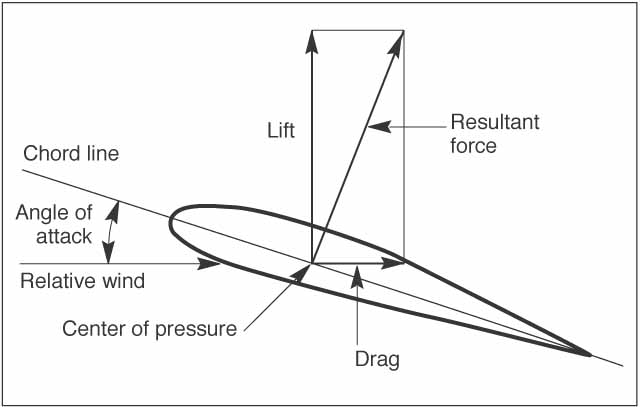
\includegraphics[width=0.332\textwidth]{figuras/aerodinamica_Figura_1a.jpg}
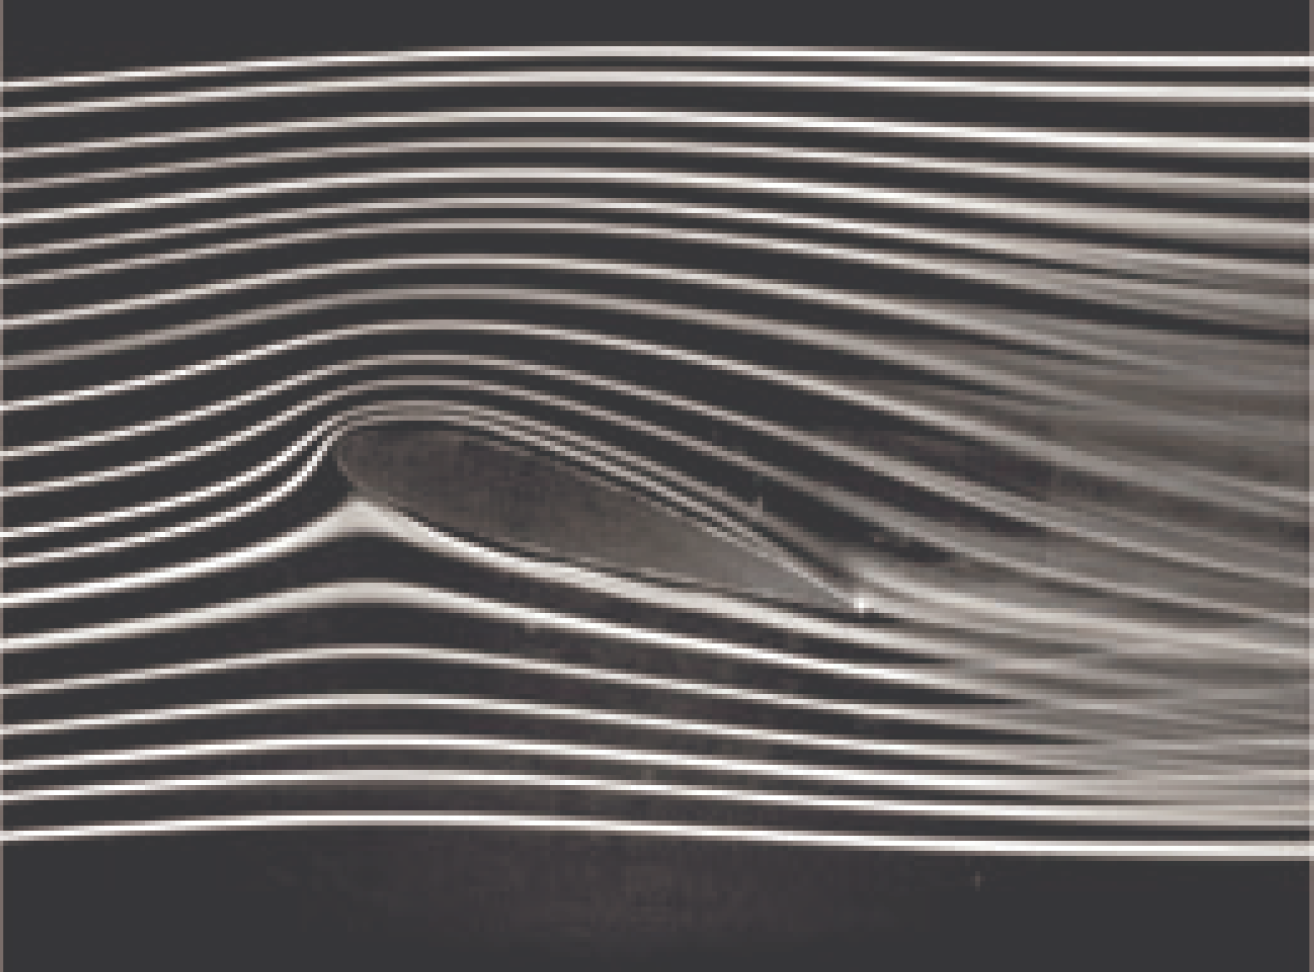
\includegraphics[width=0.284\textwidth]{figuras/aerodinamica_Figura_1b.png}
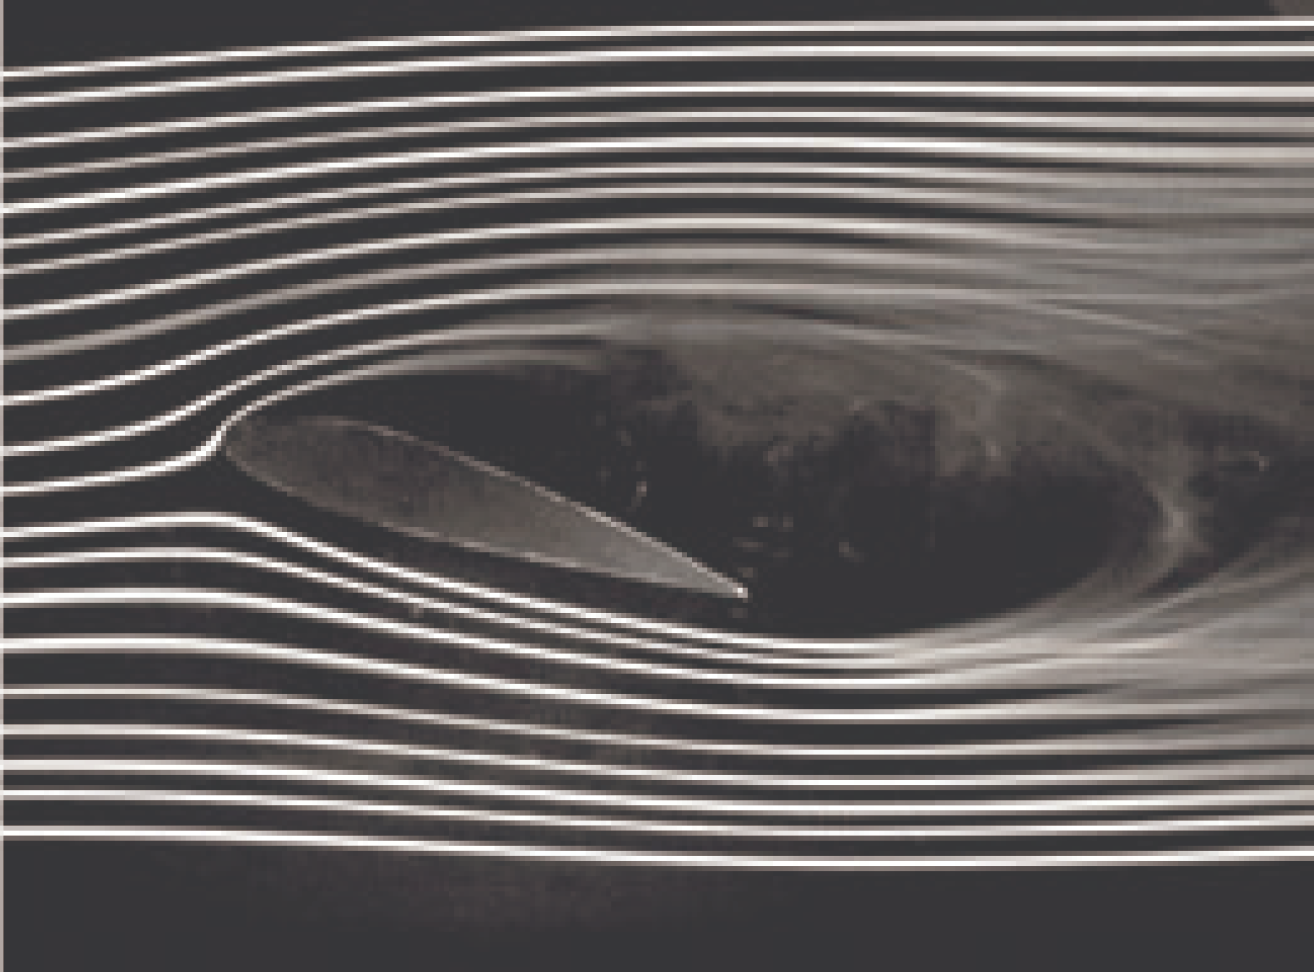
\includegraphics[width=0.284\textwidth]{figuras/aerodinamica_Figura_1c.png}
\end{center}
\vspace*{-0.6cm}
\caption[]{\label{aerofoil}{\'Angulo de ataque (izquierda). Las l\'ineas de corriente del aire siguen la superficie del ala (centro). Las l\'ineas de corriente del aire no siguen la superficie del ala, entrando en turbulencia (derecha).}}
\end{figure}

Para \'angulos de ataque peque\~nos la fuerza de elevaci\'on aumenta con el \'angulo. Sin embargo para \'angulos grandes las l\'ineas de corriente del aire se separan del ala y el movimiento se vuelve turbulento (Figura~\ref{aerofoil} derecha~\cite{babinsky}). Como consecuencia la fuerza de elevaci\'on disminuye para \'angulos mayores que un \'angulo de ataque, denominado \'angulo de atascamiento. El coeficiente de elevaci\'on, $C_e$, viene dado por $C_e = 2 F_e / (\rho v^2 S)$. Para \'angulos de ataque peque\~nos este coeficiente no depende de la velocidad.


\section{Dispositivo experimental}

Se dispone de un generador de aire regulable y un t\'unel aerodin\'amico de secci\'on variable (Figura~\ref{dispositivo} izquierda). Tambi\'en se dispone de un perfil de ala de avi\'on con un \'angulo de ataque regulable con agujeros en la parte superior e inferior (Figura~\ref{aerofoil} centro) lo que permite medir la presi\'on en distintos puntos del ala. Para medir la presi\'on se dispone de un man\'ometro de tubo inclinado (Figura~\ref{aerofoil} derecha) y de un tubo de Pitot. La fuerza de elevaci\'on se mide mediante una balanza.
%
\begin{figure}[htb]
\begin{center}
\hspace*{0.0cm}
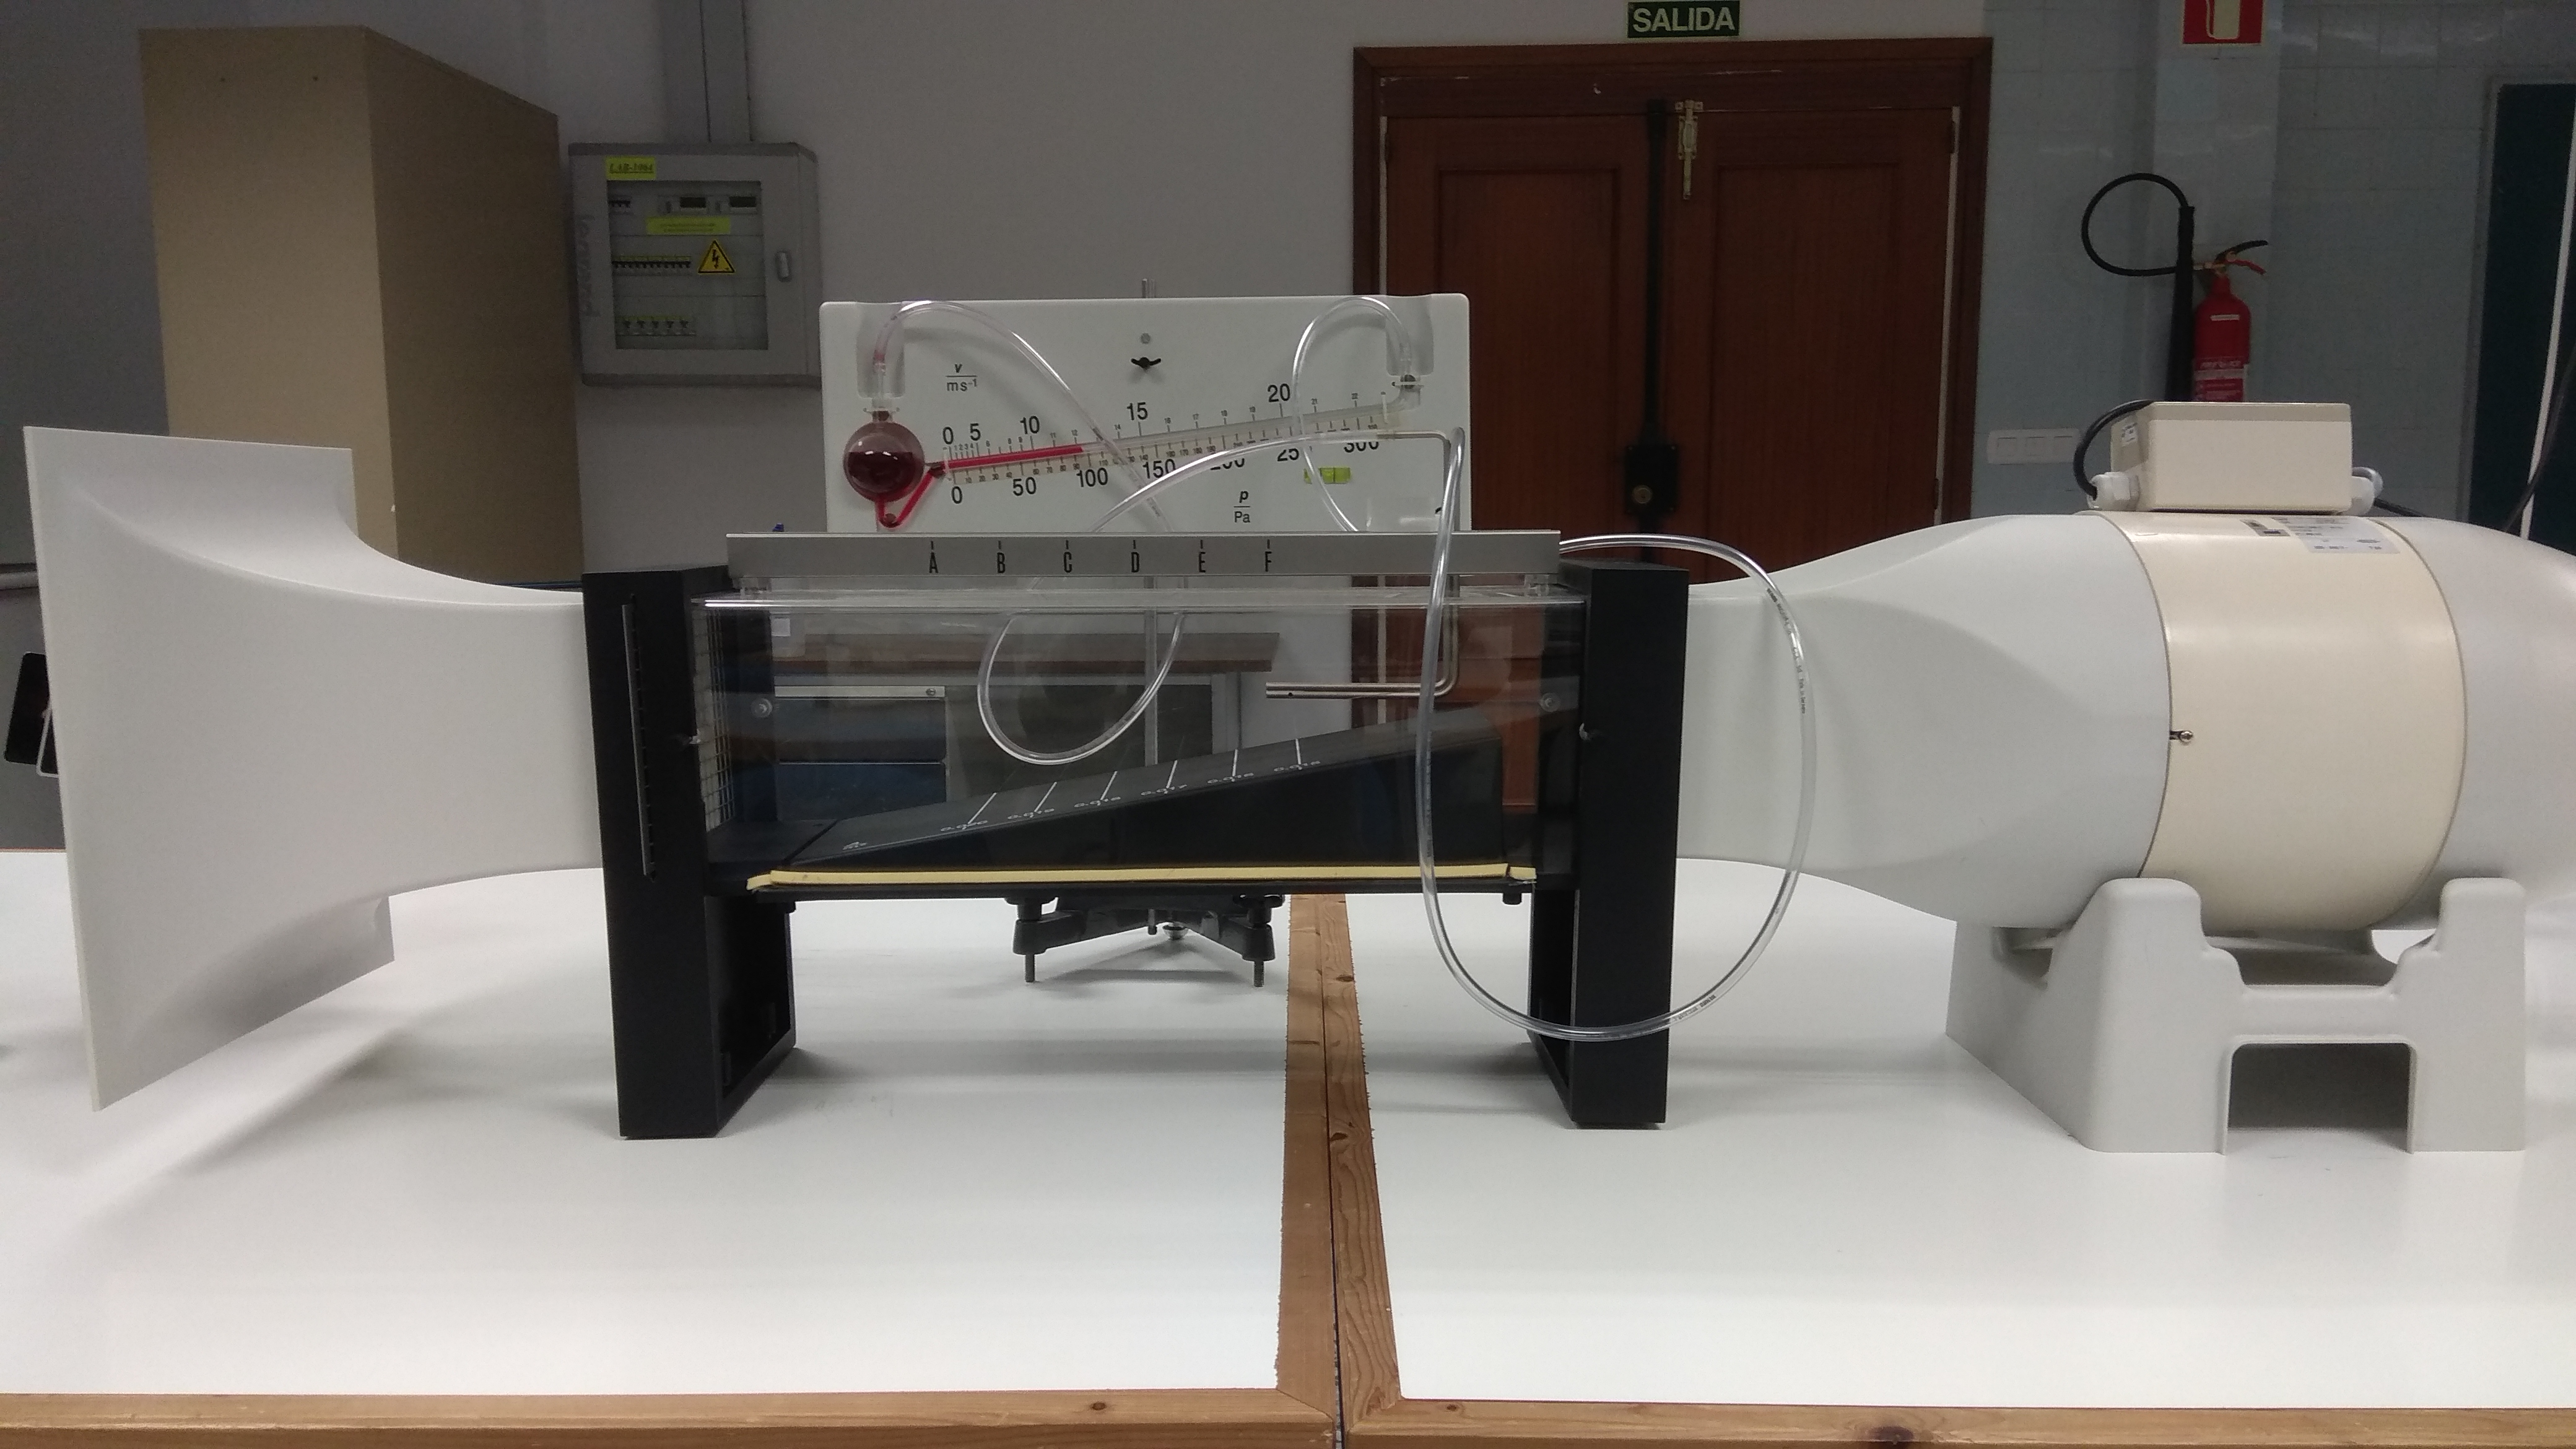
\includegraphics[width=0.552\textwidth]{figuras/aerodinamica_Figura_2a.jpg}
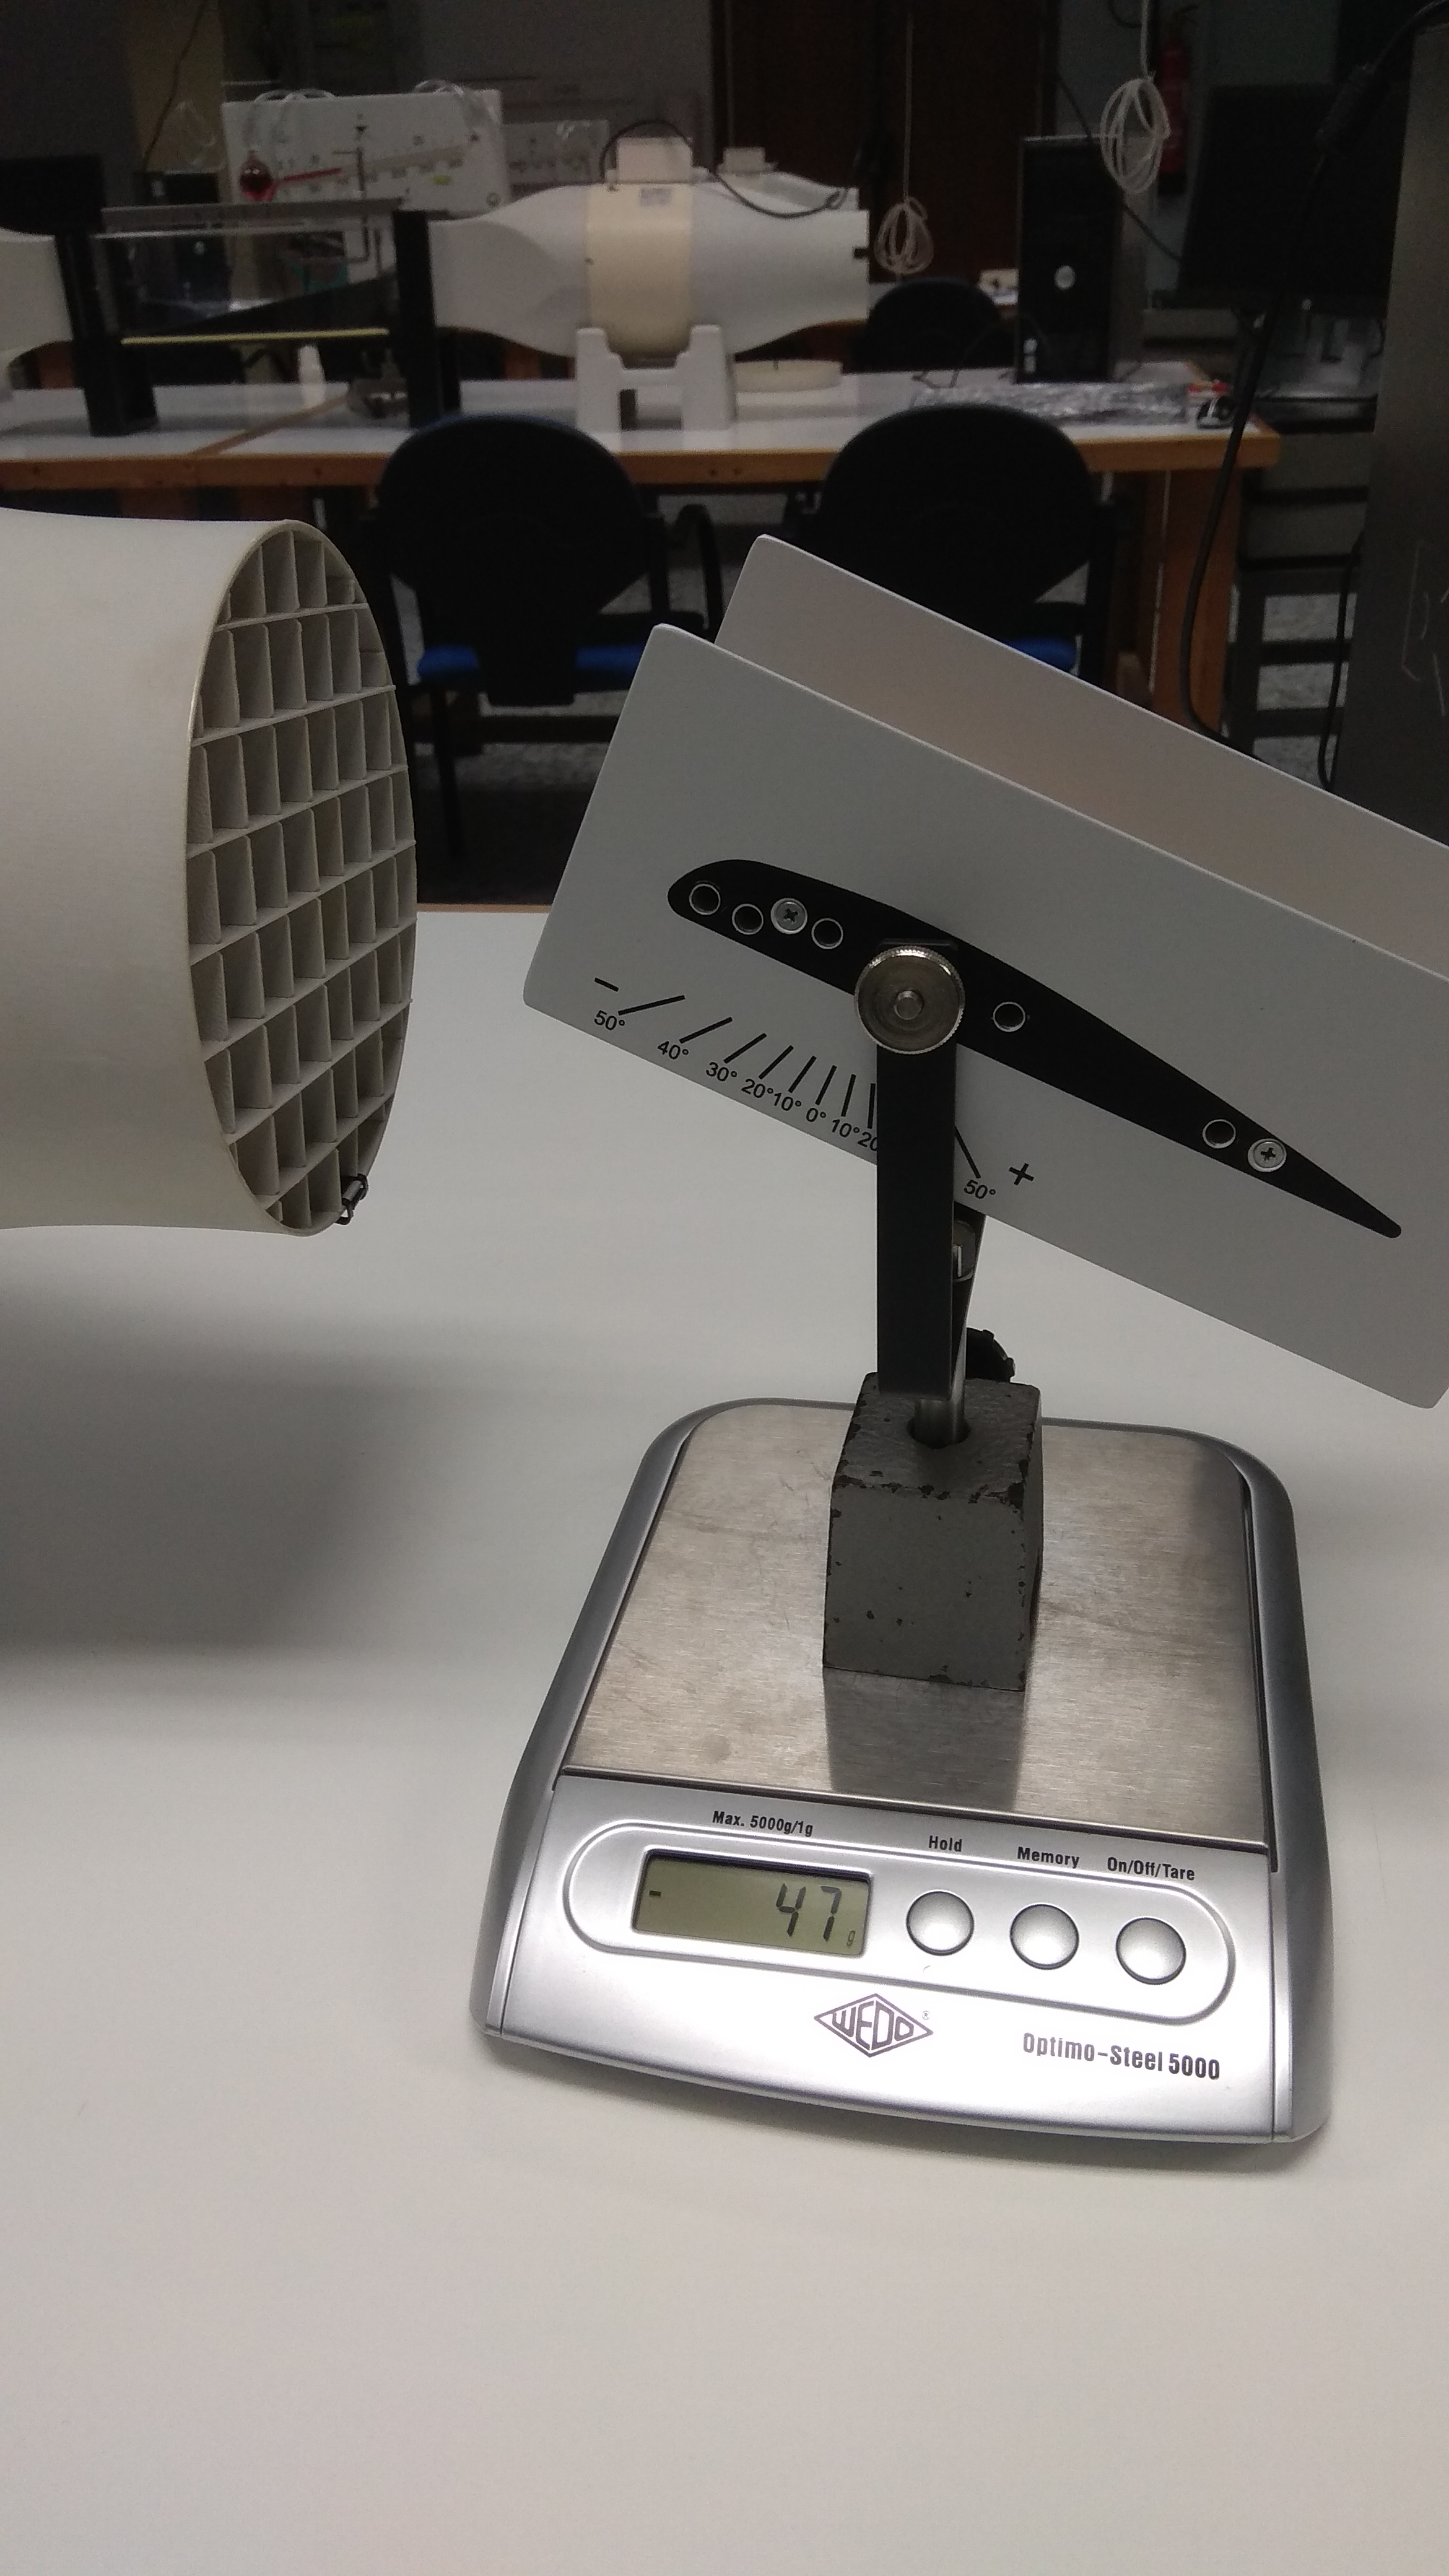
\includegraphics[width=0.174\textwidth]{figuras/aerodinamica_Figura_2b.jpg}
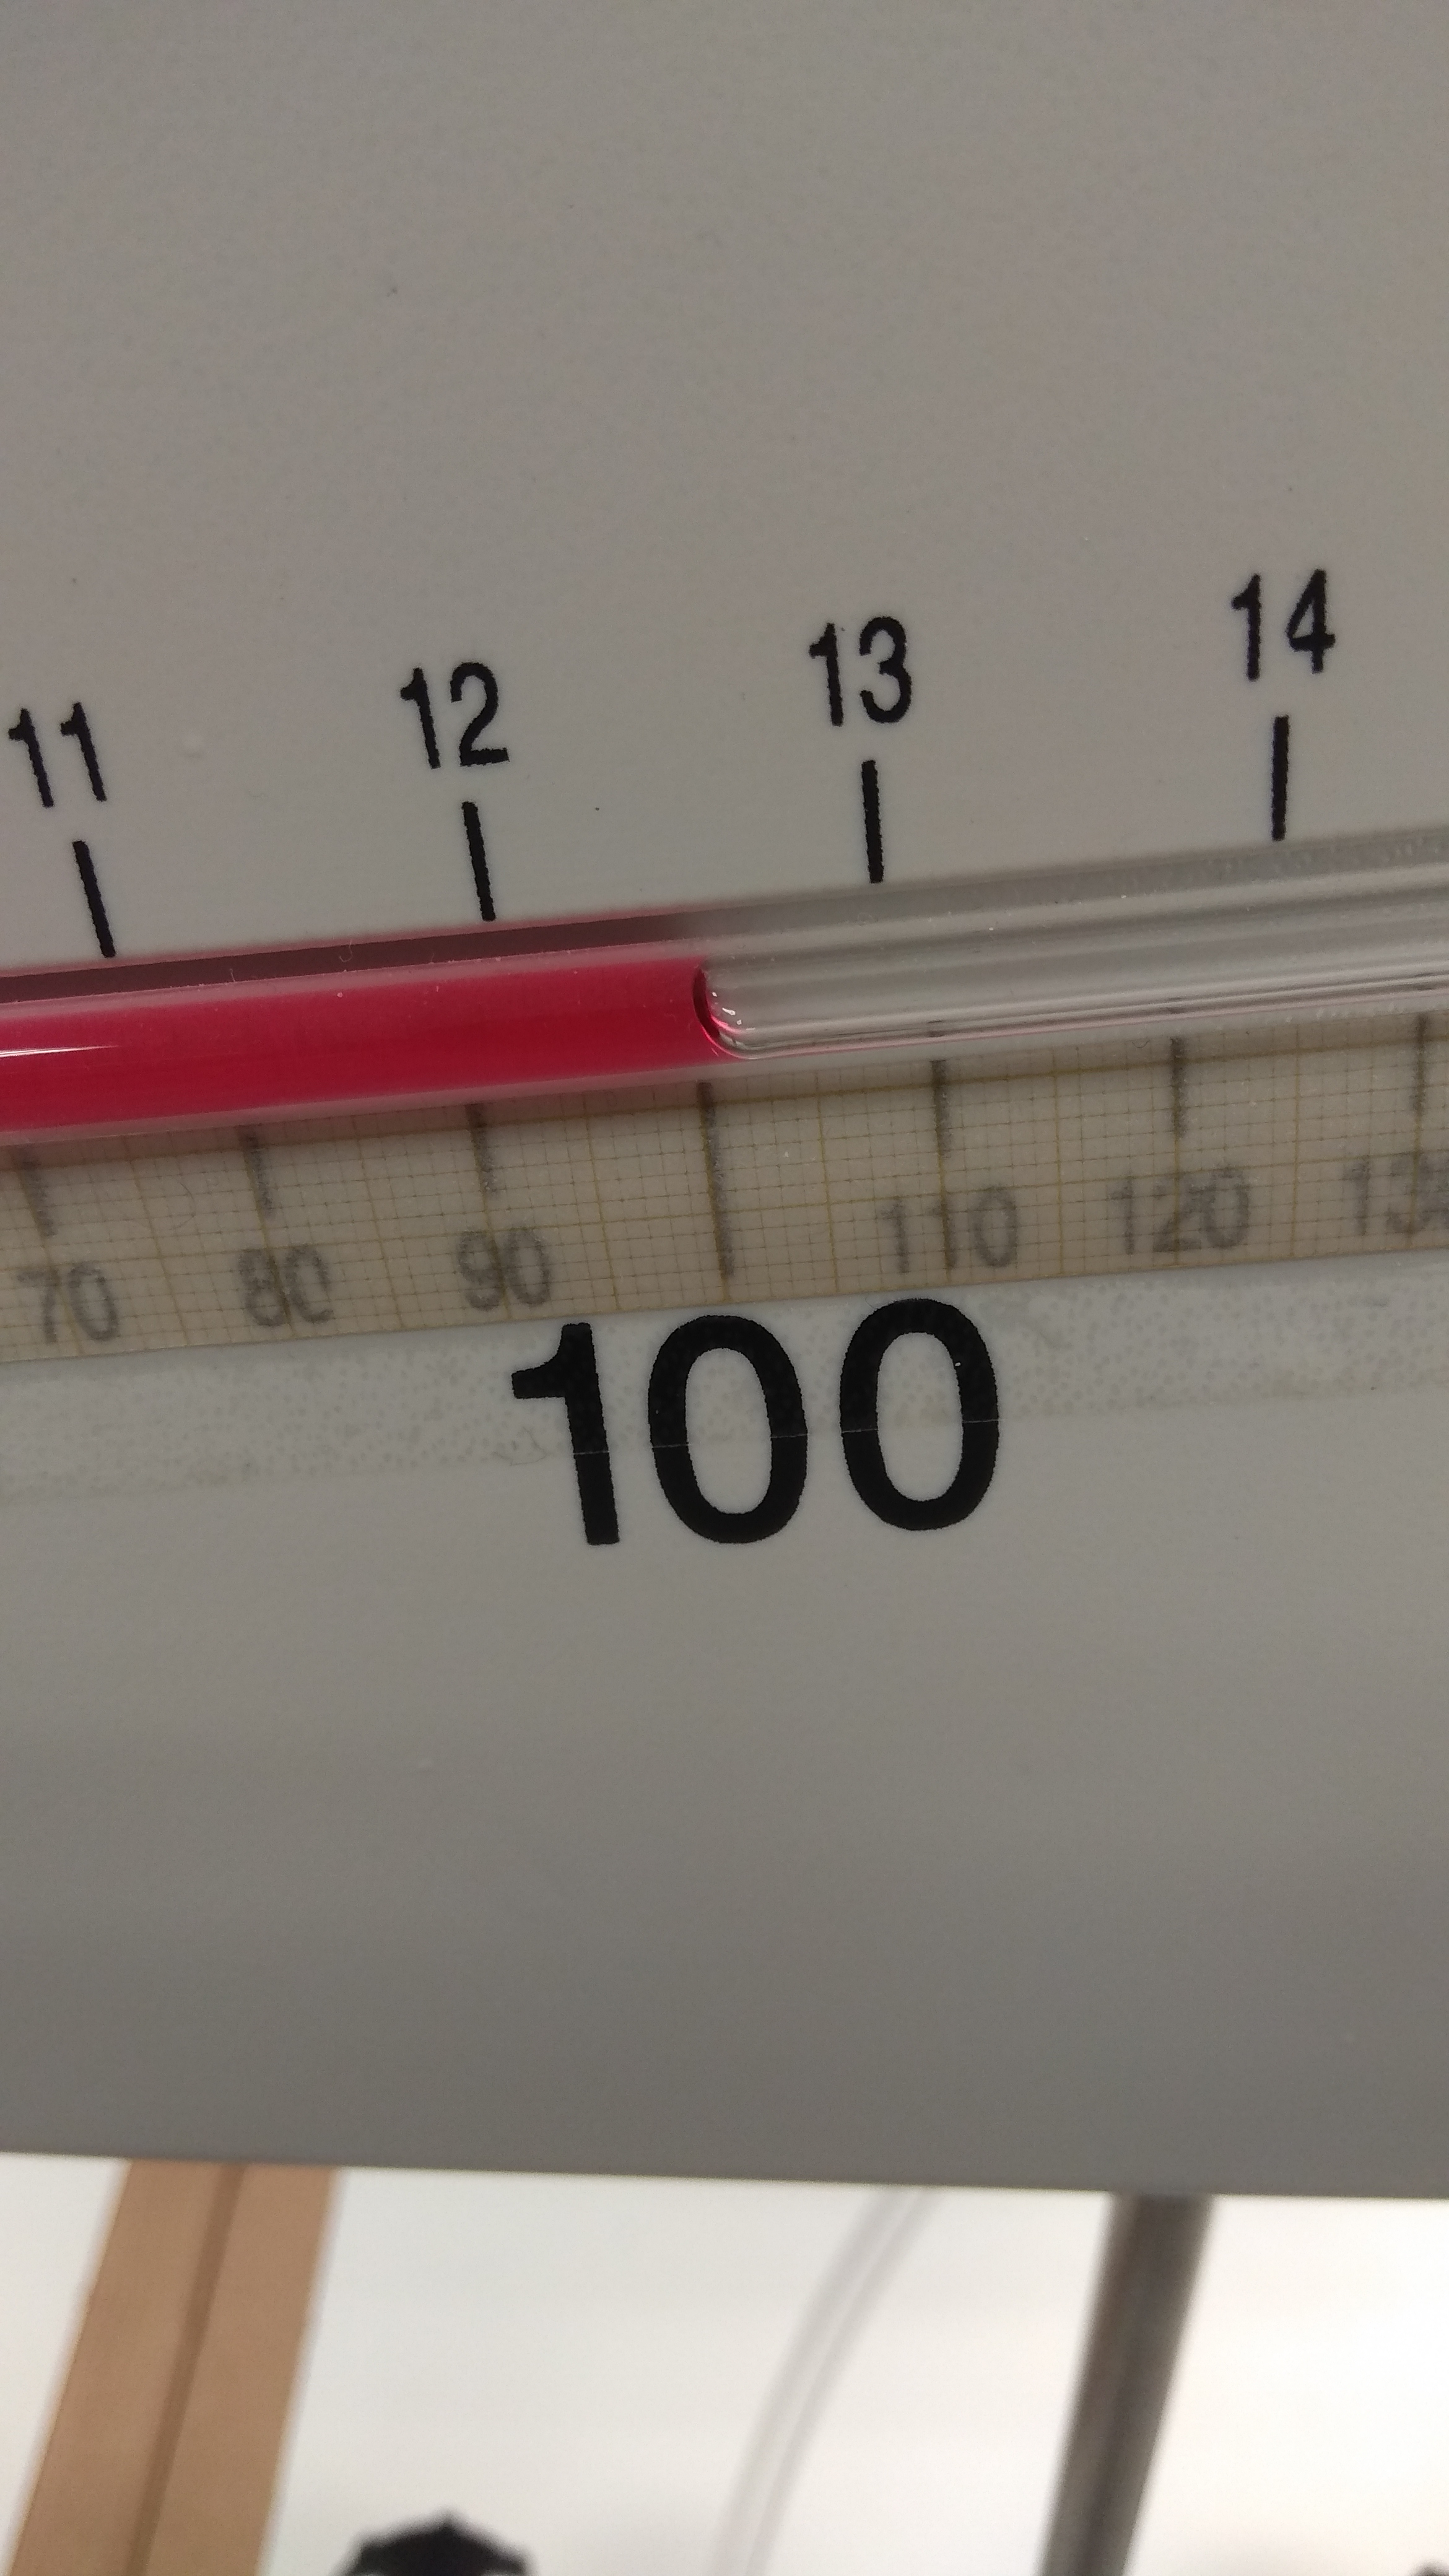
\includegraphics[width=0.174\textwidth]{figuras/aerodinamica_Figura_2c.jpg}
\end{center}
\vspace*{-0.6cm}
\caption[]{\label{dispositivo}{Generador de aire regulable y t\'unel aerodin\'amico de secci\'on variable (izquierda). Perfil de ala de avi\'on y balanza (centro). Detalle de la muesca del l\'iquido del man\'ometro de tubo inclinado (derecha).}}
\end{figure}


\section{Desarrollo}

\subsection{T\'unel aerodin\'amico}

En la primera parte se utiliza un t\'unel aerodin\'amico de secci\'on variable para obtener la presi\'on total y el caudal para distintas secciones, lo que permite comprobar la ecuaci\'on de Bernoulli. Si la altura es constante se obtiene que el valor de la velocidad es
%
\begin{equation*}
v = \sqrt{\frac{2(p_t - p)}{\rho}},
\end{equation*}
%
donde $p_t$ es la presi\'on total,  $p$ es la presi\'on est\'atica y $\rho = 1,2~{\rm kg/m^3}$ es la densidad del aire. Utiliza en esta parte la potencia m\'axima del generador. Mide la presi\'on total con el tubo de Pitot en las posiciones del t\'unel aerodin\'amico para las que se indica la secci\'on $A$. La presi\'on en el tubo con agujero lateral es $p_t = p + \rho v^2 / 2$, mientras que la presi\'on en el tubo con agujero en la punta es la presi\'on est\'atica $p$. Analiza si la presi\'on total $p_t$ es constante. El caudal $C = Av$ se obtiene calculando la velocidad del aire a partir de la medida de la diferencia de presiones en las posiciones del t\'unel aerodin\'amico para las que se indica la secci\'on $A$. Analiza si el caudal es constante en las diferentes posiciones del t\'unel y determina el valor del caudal.

\subsection{Perfil de ala}

Cuando hayas terminado esta parte el profesor montar\'a el ventilador como soplador con el perfil de ala de avi\'on. Para la potencia m\'axima del generador utiliza la balanza para medir la fuerza de elevaci\'on $F_e$ para los \'angulos de ataque $\alpha \ge -20^{\circ}$. Determina el \'angulo de atascamiento para el que la fuerza de elevaci\'on es m\'axima. Repite las medidas de la fuerza de elevaci\'on para una potencia menor del generador; para esta potencia obt\'en la velocidad del aire $v$ que produce el generador a partir de la diferencia de presiones $p_t - p$ medida con el tubo de Pitot. Repite la medida de la velocidad del aire para la potencia m\'axima del generador. Calcula el coeficiente de elevaci\'on $C_e = 2 F_e / (\rho v^2 S)$ con su error, donde $S = 0,016~{\rm m^2}$ es el \'area del ala, para los \'angulos de ataque $\alpha \geq -20^{\circ}$ y las dos potencias del generador. Representa en una misma gr\'afica $C_e$ con su error frente al \'angulo de ataque para las dos potencias del generador. Compara los resultados y com\'entalos.

Para la potencia m\'axima del generador mide la presi\'on en los agujeros de la parte superior e inferior del perfil para el \'angulo de atascamiento. Estima la fuerza de elevaci\'on a partir de estas medidas de la presi\'on y del \'area del ala $S$. Ten en cuenta que la presi\'on en cada punto es la fuerza normal a la superficie en ese punto por unidad de \'area. Compara con la medida directa de la fuerza de elevaci\'on.

\newpage
\section*{Comprueba que has incluido en el cuaderno de laboratorio y/o en el informe}

\subsection*{T\'unel aerodin\'amico}

\begin{itemize}

\item{Diferencia entre la presi\'on total y la presi\'on atmosf\'erica con su error para diferentes secciones. Comprueba si es constante.}
\item{Velocidad y caudal con sus errores para diferentes secciones. Comprueba si el caudal es constante}
\item{Valor del caudal con su error.}

\end{itemize}

\subsection*{Perfil de ala}

\begin{itemize}

\item{Fuerza de elevaci\'on con su error para \'angulos de ataque $\alpha \geq -20^{\circ}$ y \'angulo de atascamiento para dos potencias del generador.}
\item{Velocidad del aire con su error para dos potencias del generador.}
\item{Coeficiente de elevaci\'on con su error para \'angulos de ataque $\alpha \geq -20^{\circ}$ y dos potencias del generador.}
\item{Comparaci\'on en una misma gr\'afica del coeficiente de elevaci\'on con su error frente al \'angulo de ataque para las dos potencias del generador.}

\end{itemize}

\subsection*{\'Angulo de atascamiento y potencia m\'axima del generador}

\begin{itemize}

\item{Presi\'on con su error en los agujeros de la parte superior e inferior del perfil. Esquema con la posici\'on en el perfil de los agujeros.}
\item{Estimaci\'on de la fuerza de elevaci\'on con su error a partir de estas medidas de la presi\'on.}
\item{Comparaci\'on con la medida directa de la fuerza de elevaci\'on.}

\end{itemize}


%-------------------------------------------------------------------------------
% Bibliografia
%-------------------------------------------------------------------------------

\begin{thebibliography}{X}

\bibitem{tipler}
P.~A.~Tipler y G.~Mosca,
\textit{F\'isica para la ciencia y la tecnolog\'ia}. 
Editorial Revert\'e, 2005, $5^{a}$ edici\'on, Volumen 1, Cap\'itulo 13.

\bibitem{anderson}
D.~F.~Anderson, S.~Eberhardt,
\textit{The Newtonian description of lift of a wing}.
FERMILAB-Pub-01/036-E, 2001.

\bibitem{babinsky}
H.~Babinsky,
{\it How do wings work?}
Physics Education {\bf 38}, pp. 497-503, 2003.

\end{thebibliography}


%-------------------------------------------------------------------------------
% Fin del documento
%-------------------------------------------------------------------------------

\end{document}
